\documentclass[10pt,a4paper]{article}
\usepackage[utf8]{inputenc}
\usepackage[parfill]{parskip}
\usepackage[section]{placeins}
\usepackage{subfig}
\usepackage{graphicx}
\usepackage{array}
\usepackage{tabularx}
\usepackage[scientific-notation=true]{siunitx}
\usepackage{amsmath}
\usepackage{hyperref}
\usepackage{epigraph}
\author{Dominik Nerger (i6146759)}
\title{Text Mining South Park}
\date{\today}

\begin{document}
	\maketitle
	
	\tableofcontents
	\newpage
	\clearpage
	\setcounter{page}{1}
	\section{Introduction}
	\epigraph{ And tell everyone in the past for us, that no one single answer... is ever the answer. }{UAA Leader, Ep. Go God Go XII}

	South Park is an animated series revolving around the four boys Stan Marsh, Kyle Broflovski, Eric Cartman and Kenny McCormick who live in South Park, Colorado. South Park has the third most episodes in regard to American animated TV series, totaling 277 episodes over 20 seasons. 
	
	Because of the huge amount of episodes, it is an interesting target for the practical assignment, which is part of the course \textit{Information Retrieval \& Text Mining}, with the possibility of acquiring new insights into a TV series that is used to satirize American culture. 
	
	At first, all libraries that were used will be presented. Afterwards, the data set and the used corpora are introduced.  Then the pre-processing tasks that are performed on the data set will be explained. Next, the results and visualization will be discussed while explaining why and how everything has been implemented.
	In the end, a conclusion will be drawn and possible improvements for the future will be discussed.	
	
	
	The repository is available on GitHub\footnote{\url{https://github.com/dnerger/South-Park-Text-Mining}}.
	\section{Libraries}
	
	All scripts have been programmed in \textit{R}. To execute the scripts, R needs to be installed. To view temporary files that are executed during runtime, e.g. the corpus or a TermDocumentMatrix, it is advised to install RStudio. The libraries necessary for each script are imported at the top of each script, if they are not installed they can be installed by executing:
	
	\begin{verbatim}
	install.packages("library-name")
	\end{verbatim}
	
	In the following, all libraries that are related to Text Mining techniques will be introduced shortly.
	
	The library \textbf{tm} is the Text Mining package of R, which enables pre-processing of data sets and allows to build the corpus. \textbf{RWeka} is a collection of machine learning algorithms for data mining tasks. \textbf{NMF} introduces the Non-negative Matrix Factorization to R.
	\textbf{NLP} and \textbf{OpenNLP} are libraries that provide Natural Language Processing techniques and are used for NER-Tagging. \textbf{syuzhet} uses tokenized input to extract sentiments and emotions and contains the three dictionaries \textit{bing}, \textit{afinn} and \textit{nrc}.
	The package \textbf{stm} is used for Structural Topic Modeling  which is LDA with additional met-data and can be visualized using the package \textbf{LDAvis}.
	Libraries used for visualization include \textbf{igraph},\textbf{ggplot2}, \textbf{ggraph}, \textbf{viridis} and \textbf{wordcloud}.
	
	\section{Data set}	
	The data set spans from seasons \textbf{1} to \textbf{18}, adding up to 257 episodes overall with a file size of 5.41MB. It contains 70896 rows, with each row possessing information about the \textbf{season}, \textbf{episode}, \textbf{character} and \textbf{line} and is available as a \textit{.csv} file.
	
	The data set has been crawled by Bob Adams and is available to download on GitHub\footnote{\url{https://github.com/BobAdamsEE/SouthParkData}}. It has been assembled by crawling the South Park Archives\footnote{\url{http://southpark.wikia.com/wiki/South_Park_Archives}}. The code of this GitHub repository is not available to the public.
	
	 I made an attempt at a crawl with the R package \textbf{rvest}, which is able to harvest data from websites.  However, the \textit{html data} of the episode scripts provided on the South Park Archives differ between episodes. For 16 of 20 seasons, the whole episode needs to be pre-processed manually because the \textbf{line} and \textit{character} are extracted individually and can not be merged because of random whitespace lines that are introduced by \textbf{rvest}.
	 
	 In the scripts, the data set is used in three different variations:
	 \begin{enumerate}
	 \item \textit{dialogue} - each entry holds information about season, episode, character and line
	 \item \textit{by.season} - each entry holds information about season and the complete script for that season
	 \item \textit{by.episode} - each entry holds information about that episode, season and script for that episode
	 \end{enumerate}
	 
	 Both \textit{by.episode} and \textit{by.season} are created by using the data from \textit{dialogue}.
	
	
	
	
	\section{Pre-processing}
	In general, the standard pre-processing tasks are executed on the corpus. Depending on the later use, different packages perform these.
	The package \textbf{tm} is used to convert the corpus to lower case, remove punctuation and numbers as well as strip whitespaces. Furthermore, stopwords are removed using the stopword list from the Snowball stemmer project. The corpus is stemmed using Porter's stemming algorithm.\footnote{\url{http://snowball.tartarus.org/algorithms/english/stop.txt}} It is used together with several DocumentTerm- and TermDocument-Matrices. From these DTMs/TDMs, sparse terms are removed. The maximum allowed sparsity depends on the data set and the intended use, with the allowed percentage being higher for the \textit{by.episod} data set in comparison to \textit{by.season} because there are more documents in the \textit{by.episode} data set. 
	
	The pre-processing for the Structural Topic Model is done with the same tasks, however those are performed by the package \textbf{stm} itself.
	
	For the Named Entity Recognition with package \textbf{openNLP}, no pre-processing tasks are performed. They can be executed and might improve the overall runtime, but it does not change the overall result. Especially stemming and the lower case convertion could decrease the results because stemmed or lower case entities, as well as the sentiments that are mined, will not be recognized.

	
	
	\section{Results and visualization}
	
	To sufficiently present the results and the corresponding visualization, each relevant script will present them in their own subsection.
	
	\subsection{Wordclouds}
	To start to gain an insight into South Park, I started with building wordclouds that display the most frequent words to see what South Park is about. However, even with stopwords removed, the words that are most frequent mostly include words such as \textit{get, just} and \textit{now}. From these words, nothing about the TV show can be derived. 
	
	To get meaningful answers to what is important in and characteristic for South Park, the corpus is built with a term frequency-inverse document frequency (tf-idf) weight, which reflects how important each term is to the corresponding document in the corpus.
	\begin{figure}[!h]
  \centering
  \begin{minipage}[b]{0.45\textwidth}
    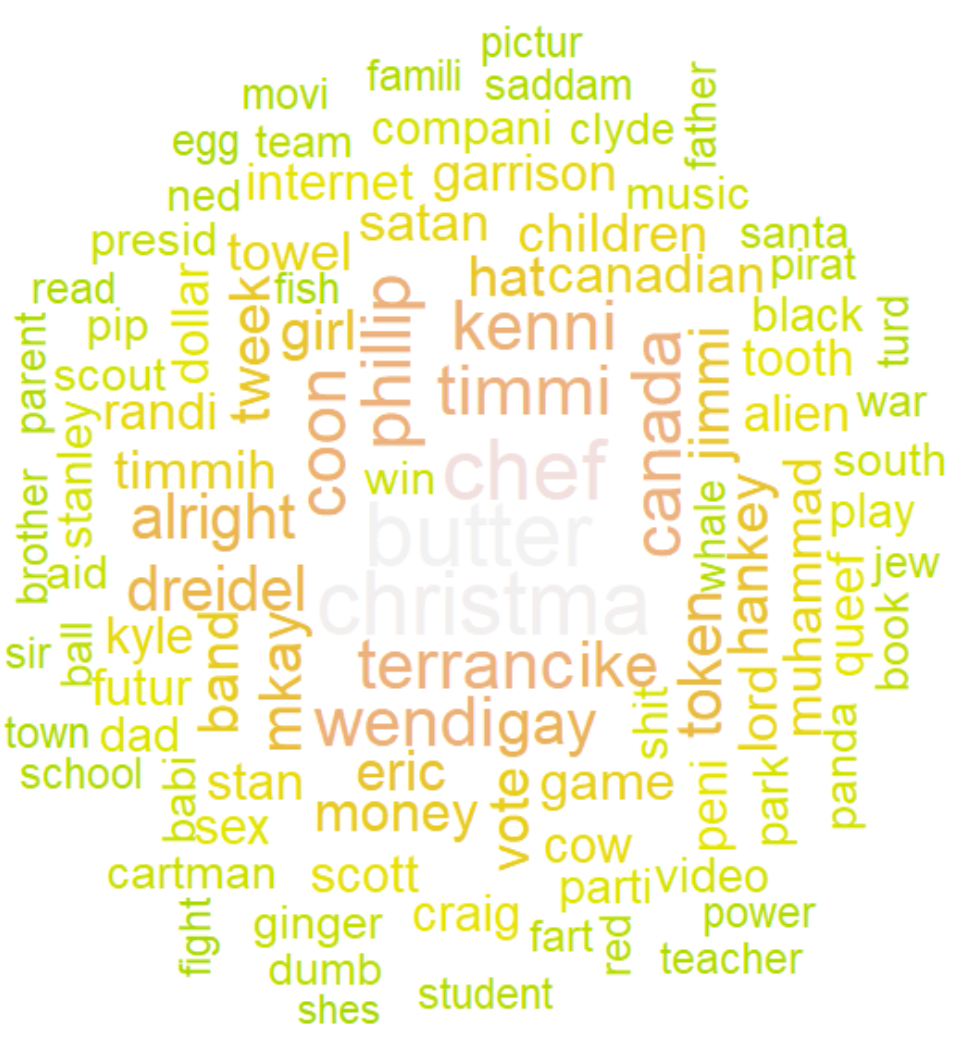
\includegraphics[width=\textwidth]{images/WordCloud-TFIDF-episode.png}
    \caption{ Terms with highest TF-IDF score - \textit{by.episode}}
	\label{fig:WordCloud-TFIDF-ep}
  \end{minipage}
  \hfill
  \begin{minipage}[b]{0.5\textwidth}
    \includegraphics[width=\textwidth]{images/WordCloud-TFIDF.png}
    \caption{Terms with highest TF-IDF score - \textit{by.season}}
	\label{fig:WordCloud-TFIDF-s}
  \end{minipage}
\end{figure}
	
	With this weighting, the terms that are most important over all 18 seasons can be derived, as can be seen in Figures~\ref{fig:WordCloud-TFIDF-ep} and~\ref{fig:WordCloud-TFIDF-s}.
	
		The difference between the wordclouds descends from the different \textit{idf} weights for the data sets \textit{by.season} and \textit{by.episode}. The words in Figure~\ref{fig:WordCloud-TFIDF-ep} show the names of secondary characters such as Butters, Kenny and Wendy. These characters are not featured in Figure~\ref{fig:WordCloud-TFIDF-s} since they do appear in every season, but not in every episode.
		
			\begin{figure}[h]
	\centering
	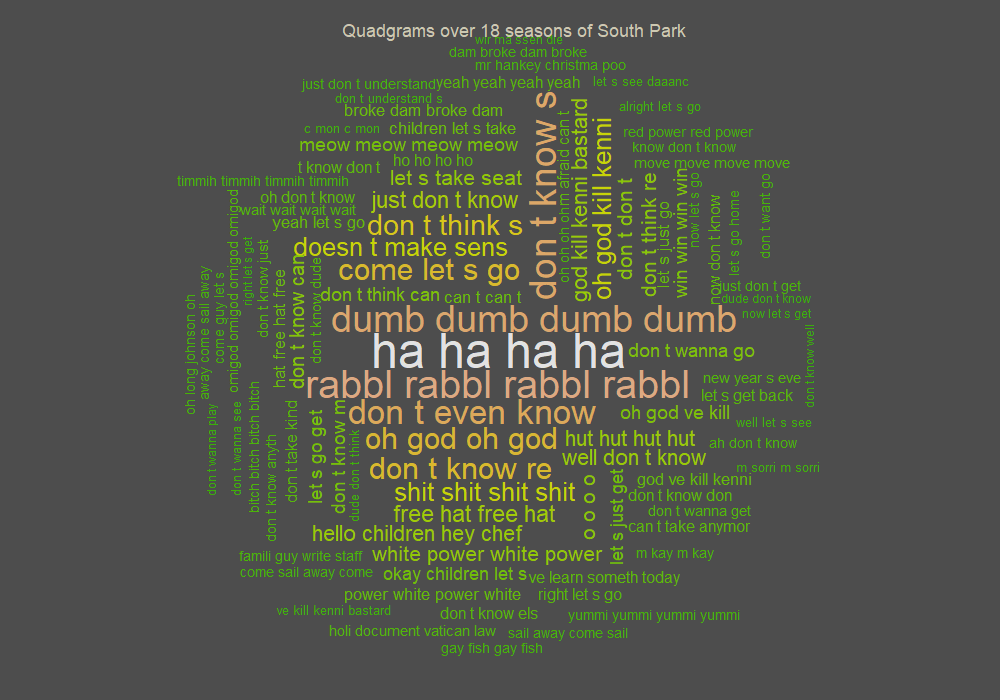
\includegraphics[scale=0.5]{images/WordCloud-ngram.png}
	\caption{Wordcloud containing ngrams (n=4) by frequency}
	\label{fig:WordCloud-ngram}
	\end{figure}
		
		Figure~\ref{fig:WordCloud-ngram} shows the most frequent quadgram phrases without stopwords included. This includes sentences like the trademark phrase "Oh my god, they killed Kenny", which is shown as "oh god kill kenni".

	
	
	\subsection{Co-occurences and dendrogram}
	To gain insight into the relations between characters and to confirm the major characters of South Park, which are Stan, Kyle and Cartman, I decided to visualize the 20 characters with the most lines.
	
	As can be seen in Figure~\ref{fig:SpeakingPercentage}, Cartman is the character with most lines overall, with Stan and Kyle, as well as Butters and Randy being other major characters.
	
	\begin{figure}[h]
	\centering
	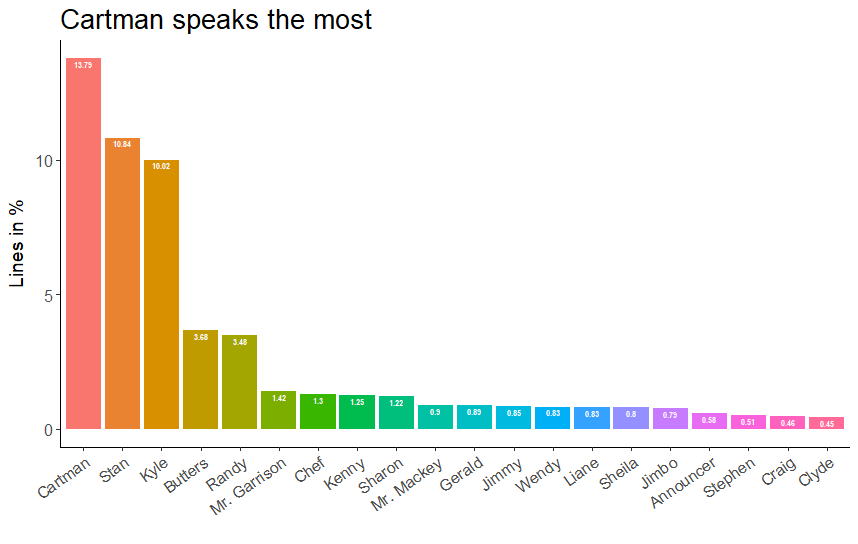
\includegraphics[scale=0.5]{images/speakingPercentage.png}
	\caption{Speaking percentage for 20 major characters}
	\label{fig:SpeakingPercentage}
	\end{figure}	
	
	
	However, this does not show the relations between the characters. To visualize this, I decided to create a co-occurence network by creating a DocumentTermMatrix that contains the characters as terms and the unique episode number as document. The value in each entry is the amount of lines for the character in the specific episode. By using the formula $C = A^tA$ with A as the DocumentTermMatrix, I created a TermTermMatrix that contains the co-occurences between lines of characters, resulting in the co-occurences of the 20 most relevant characters in South Park.
	
	
	\begin{figure}[h]
	\centering
	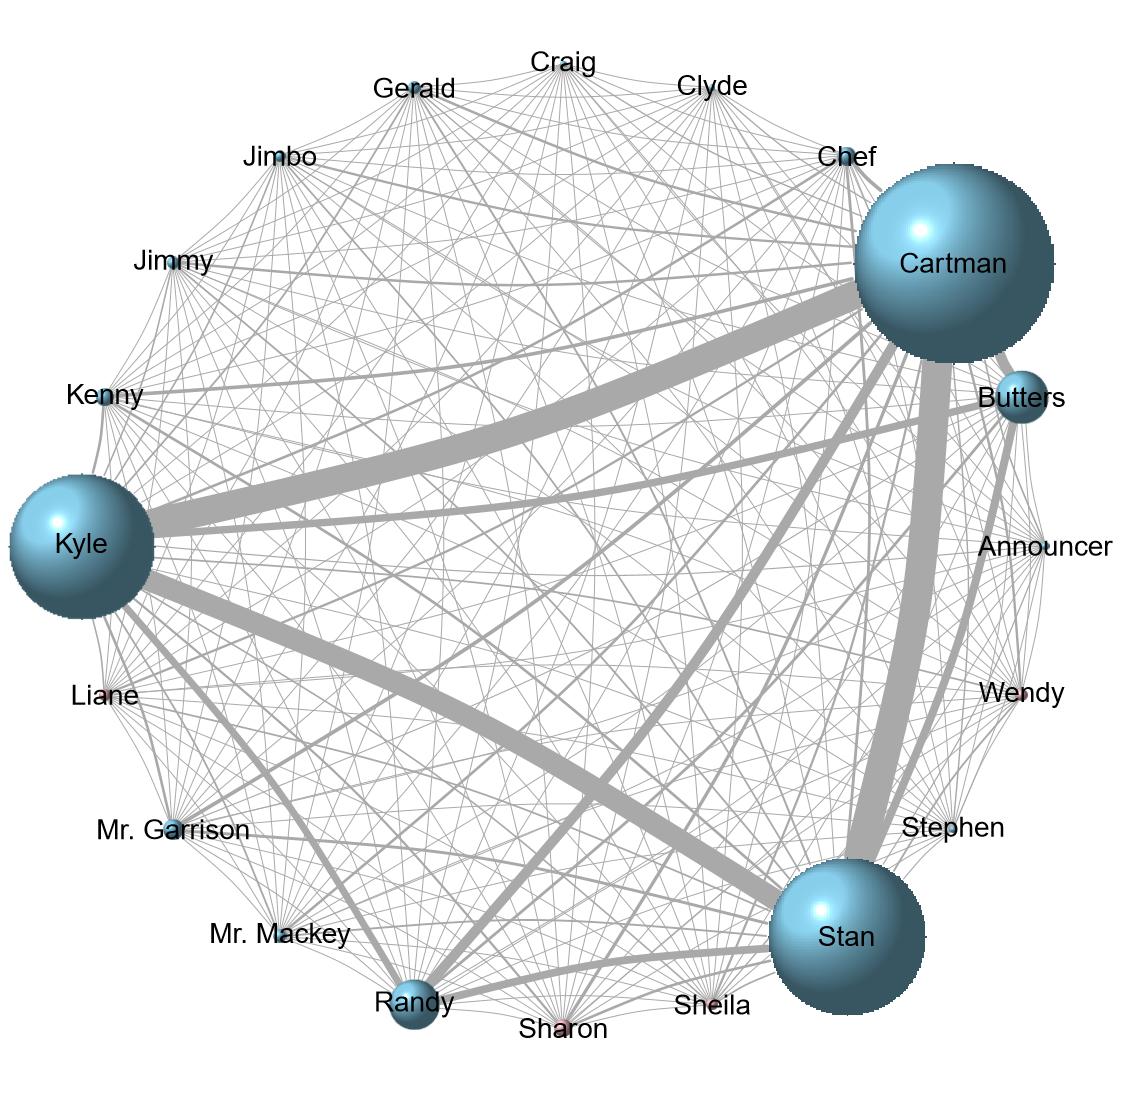
\includegraphics[scale=0.6]{images/CoOccurenceMatrix.png}
	\caption{Co-occurence network}
	\label{fig:CoOccurence}
	\end{figure}		
	
	
	As can be seen in Figure~\ref{fig:CoOccurence}, all 20 major characters interact in some way throughout all 257 episodes, with Cartman, Kyle and Stan being characters that are closely tied together. 
	
	Since it is hard to derive the relations between the characters from Figure~\ref{fig:CoOccurence}, I decided to use a cluster dendrogram to visualize which characters have the most episodes in common.
	
	Figure~\ref{fig:Dendrogram} shows the dendogram clustering the characters. The further down the node of two characters splits, the more episodes these characters have in common. This shows once again that the major characters Cartman, Stan and Kyle are closely tied together. Furthermore, interesting connections between the students Clyde and Craig as well as 
	
		\begin{figure}[h]
	\centering
	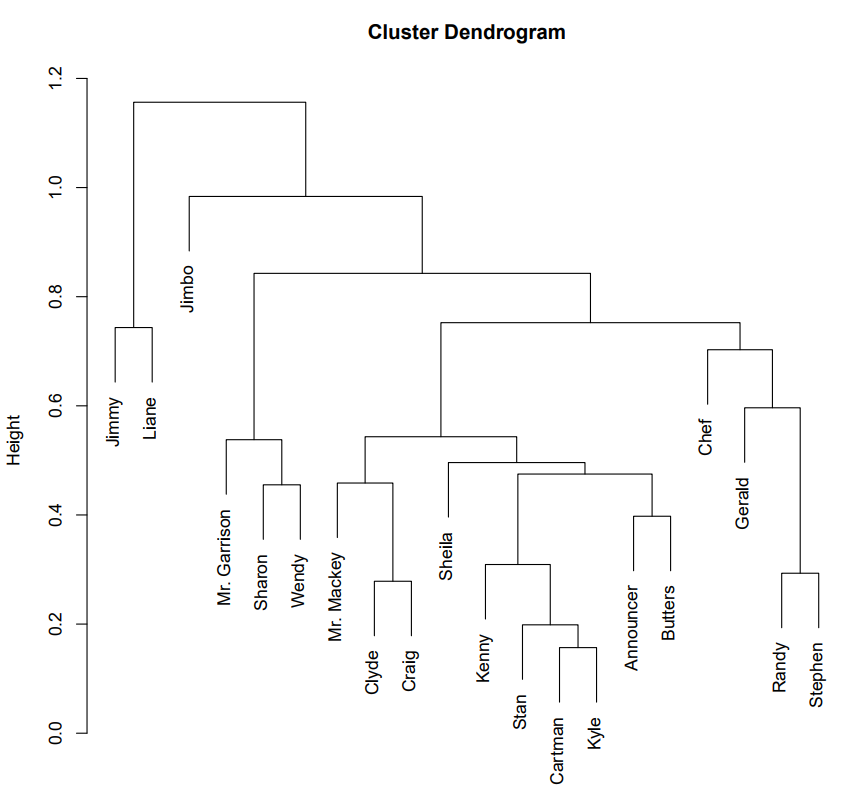
\includegraphics[scale=0.4]{images/Dendrogram.png}
	\caption{Cluster dendrogram of 20 major South Park characters}
	\label{fig:Dendrogram}
	\end{figure}
	\FloatBarrier
	\newpage
	
	\subsection{Named Entity Recognition}
	To extract information about characteristic information such as organizations, persons and locations that are mentioned in South Park, I decided to use the Named Entity Recognition provided by the Apache \textbf{openNLP} library.
	
	\subsection{Sentiment and Emotion Mining}
	Another approach to learn something about South Park is to extract the sentiments and emotions that are expressed by the characters. The sentiments are annotated onto the seasons, using ...
	
	After the complete corpus has been annotated, which results in little chunks of words being tied together, the sentiments are processed with the library \textbf{syuzhet} and the sentiment dictionary \textit{nrc}.
	During the processing the word chunks are grouped with 100 chunks being tied together. Under the assumption that each character line contains at least 1 chunk, this results in a minimum of 700 grouped chunks for 70000 character lines, which can be seen as roughly three different sentiment values for each episode. This enables a nice visualization of 
		
	
	
	\section{Conclusion}
	In conclusion, 

	\section{Future work}
\end{document}
